\documentclass[12pt, letterpaper]{article}
\usepackage[top=2.5cm, bottom=2.5cm, left=3cm, right=2.5cm]{geometry}
\usepackage[utf8]{inputenc}
\usepackage[T1]{fontenc}
\usepackage{lmodern}
\usepackage{amsmath, amssymb}
\usepackage{booktabs}
\usepackage{tabularx}
\usepackage{longtable}
\usepackage{array}
\usepackage{multirow}
\usepackage{xcolor}
\usepackage{graphicx}
\usepackage{float}
\usepackage{listings}
\usepackage[most, breakable]{tcolorbox}
\usepackage{enumitem}
\usepackage{fancyhdr}
\usepackage{titlesec}
\usepackage{setspace}
\usepackage{microtype}
\usepackage[hidelinks]{hyperref}
\usepackage{parskip}
\usepackage{pgfplots}
\pgfplotsset{compat=1.15}
\usepackage{tikz}
\usepackage{graphicx}

% Colours
\definecolor{econblue}{RGB}{31,78,121}
\definecolor{researchgreen}{RGB}{21,101,45}
\definecolor{exampleorange}{RGB}{180,80,20}
\definecolor{lightgray}{RGB}{245,245,245}
\definecolor{boxblue}{RGB}{220,235,248}

% Section headings
\titleformat{\section}{\large\bfseries\color{econblue}}{\thesection}{1em}{}%
  [\vspace{-4pt}\rule{\linewidth}{0.4pt}]
\titleformat{\subsection}{\normalsize\bfseries\color{econblue}}{\thesubsection}{1em}{}
\titleformat{\subsubsection}{\normalsize\bfseries}{\thesubsubsection}{1em}{}

% Page style
\pagestyle{fancy}
\fancyhf{}
\fancyhead[L]{\small\itshape ECON 230 --- Introduction to Behavioural Economics}
\fancyhead[R]{\small\itshape Chapter 9: Choice Architecture}
\fancyfoot[C]{\small\thepage}
\renewcommand{\headrulewidth}{0.4pt}
\setlength{\headheight}{14pt}

% tcolorbox styles
\tcbuselibrary{breakable, skins, listings}

\newtcolorbox{researchbox}{
  enhanced, breakable,
  colback=researchgreen!6, colframe=researchgreen!55,
  title=\textbf{Research Study},
  fonttitle=\bfseries\small,
  attach boxed title to top left={yshift=-2mm, xshift=6mm},
  boxed title style={colback=researchgreen!55, colframe=researchgreen!55},
  before upper={\setlength{\parskip}{4pt}}
}

\newtcolorbox{examplebox}[1]{
  enhanced, breakable,
  colback=exampleorange!6, colframe=exampleorange!45,
  title=\textbf{#1}, fonttitle=\bfseries\small
}

\newtcolorbox{keybox}{
  enhanced, colback=boxblue, colframe=econblue!70,
  fontupper=\small
}

% ASCII figure style
\lstset{
  basicstyle=\scriptsize\ttfamily,
  breaklines=false,
  keepspaces=true,
  columns=flexible,
  frame=single,
  backgroundcolor=\color{lightgray},
  xleftmargin=4pt, xrightmargin=4pt,
  aboveskip=6pt, belowskip=6pt
}

% Lists
\setlist[itemize]{leftmargin=1.5em, itemsep=2pt, topsep=4pt}
\setlist[enumerate]{leftmargin=1.5em, itemsep=2pt, topsep=4pt}
\onehalfspacing

\newcolumntype{Y}{>{\raggedright\arraybackslash}X}

\begin{document}

\begin{titlepage}
\centering\vspace*{3cm}
{\Large\bfseries\color{econblue} ECON 230 --- Introduction to Behavioural Economics\\[1em]}
{\large\bfseries Course Textbook\\[2em]}
{\LARGE\bfseries\color{econblue} Chapter 9\\[0.5em]}
{\Large\bfseries Choice Architecture --- Nudges and Libertarian Paternalism\\[2em]}
\vfill
{\normalsize University of Northern British Columbia\\
Instructor: Prof.\ Muhebullah Karimzada\\
Term: Winter 2027}
\end{titlepage}
\tableofcontents
\newpage


\medskip


\section*{Chapter Overview}
\addcontentsline{toc}{section}{Chapter Overview}


The preceding eight chapters of this textbook have built a detailed picture of human decision-making that diverges sharply from the rational agent of standard economic theory. People rely on heuristics that produce systematic biases. They evaluate outcomes relative to reference points and weight losses more heavily than equivalent gains. They discount the future hyperbolically, making plans they fail to execute. They are influenced by irrelevant contextual features --- the way options are framed, the order in which they appear, the anchor provided by an arbitrary number. They follow the crowd, underreact to important information, and succumb to overconfidence.

These findings raise an obvious and urgent question: what should we do about it?

One response --- the traditional economic response --- is to insist that individuals are the best judges of their own welfare, that government intervention distorts incentives, and that people learn from experience. If someone makes bad financial decisions, the market will educate them. If someone eats unhealthily, they will suffer the consequences and adjust. The cure for bad decisions is more information, better education, and competitive markets --- not government interference in individual choice.

A second response --- drawn from behavioural economics --- is to observe that the decision environment itself powerfully influences choices, often in ways that systematically harm people, and that restructuring this environment can improve outcomes without restricting freedom. If the default on a pension plan is "not enrolled" and most workers fail to opt in --- not because they do not want retirement savings, but because inertia and present bias prevent them from acting --- then changing the default to "enrolled" preserves their freedom (they can still opt out) while dramatically improving their retirement security.

This second approach is the subject of this chapter. Richard Thaler and Cass Sunstein coined the term \textbf{libertarian paternalism} to describe the philosophy, and \textbf{nudge} to describe the specific interventions it supports. A nudge is any feature of the choice environment that alters people's behaviour in a predictable way without forbidding any options or significantly changing economic incentives. Changing a default is a nudge. Placing fruit at eye level in a cafeteria is a nudge. Sending a letter that says "nine out of ten people in your neighbourhood pay their taxes on time" is a nudge.

This chapter develops the conceptual foundations of nudge theory, describes the empirical evidence for specific nudge tools, examines the institutional structures --- particularly government "behavioural insights teams" --- that have translated these ideas into policy, and addresses the deep philosophical and ethical debates about whether nudging people toward "better" choices is compatible with respect for individual autonomy.

\medskip


\section*{Learning Objectives}
\addcontentsline{toc}{section}{Learning Objectives}


After studying this chapter, students should be able to:

\begin{enumerate}
\item \textbf{Define} a nudge precisely and distinguish it from mandates, bans, taxes, and subsidies.
\item \textbf{Explain} the concept of choice architecture and describe how default rules, ordering, framing, and salience shape decisions without altering options or prices.
\item \textbf{Describe} the organ donation default effect documented by Johnson and Goldstein (2003) and explain the mechanism responsible for it.
\item \textbf{Explain} the automatic enrolment evidence from Madrian and Shea (2001) and quantify its effect on retirement savings participation.
\item \textbf{Define} libertarian paternalism and explain how it differs from hard paternalism, soft paternalism, and the standard economic non-interventionist position.
\item \textbf{Identify} the four elements of the EAST framework (Easy, Attractive, Social, Timely) and apply them to a policy design problem.
\item \textbf{Describe} the social norm nudge mechanism and evaluate the evidence from energy conservation programmes.
\item \textbf{Explain} at least three ethical critiques of nudging --- manipulation, autonomy, and the "what counts as better" problem --- and assess their force.
\item \textbf{Identify} the major government nudge units around the world and describe the types of problems they address.
\item \textbf{Apply} nudge theory to at least two specific Canadian policy contexts and evaluate the likely effectiveness of specific interventions.
\end{enumerate}

\medskip


\section*{Introduction: The Power of the Default}
\addcontentsline{toc}{section}{Introduction: The Power of the Default}


In 1990, Austria and Germany were neighbouring countries with similar cultures, similar legal systems, similar economies, and --- on virtually every observable dimension --- similar citizens. Both countries had introduced donor card systems for organ donation in the 1970s. Both countries had the same underlying medical infrastructure, the same transplantation technology, and the same social attitudes toward donation.

There was one difference. In Germany, citizens were organ donors if and only if they had signed a donor card to opt \textit{in}. In Austria, citizens were organ donors by default and remained donors unless they took steps to opt \textit{out}.

This single difference --- which option was the default --- produced a dramatic divergence. In Germany, approximately 12\% of citizens were registered organ donors. In Austria, approximately 99.98\% of citizens were registered organ donors.

The two populations had near-identical preferences. When surveyed, citizens of both countries expressed broadly similar support for organ donation in the abstract. The difference in registration rates of nearly 90 percentage points was not produced by different preferences. It was produced by a different choice architecture: which option required action.

This is, in miniature, the central insight of behavioural policy design. The structure of the decision environment --- the \textbf{choice architecture} --- powerfully determines what people choose, independently of what they prefer. When the default is "donor," almost no one opts out, even though opting out is trivially easy. When the default is "non-donor," most people fail to opt in, even though opting in is also easy and many of them would benefit from being registered donors.

Richard Thaler, who was awarded the Nobel Memorial Prize in Economic Sciences in 2017, and Cass Sunstein, a legal scholar at Harvard Law School, synthesised this insight into a policy philosophy they called \textbf{libertarian paternalism} in a 2003 paper and developed into a book, \textit{Nudge}, in 2008. Their argument is simultaneously descriptive and prescriptive: choices are always made within a choice architecture, choice architects always influence choices, and the question is not whether to influence choices but \textit{how}.

If the cafeteria must put some food first in the line, it might as well put the fruit first. If a pension plan must have a default investment fund, it might as well be a well-diversified lifecycle fund. If a utility bill must have some design, it might as well include a comparison with neighbours' consumption. None of these arrangements restrict freedom. All of them improve outcomes --- if "better outcomes" can be defined, which, as we shall see, is itself a contested question.

\medskip


\section{Choice Architecture: The Structure of Decision Environments}



\subsection{What Is Choice Architecture?}


Every decision is made in a context. That context --- the physical environment, the sequence in which options appear, which option requires active choice and which operates by default, the way information is framed and presented, the social norms that are made salient --- is the \textbf{choice architecture}.

The term was coined by Thaler and Sunstein to draw attention to a fact that is simultaneously obvious and overlooked: someone always designs the context in which choices are made. A cafeteria manager decides where to place each food. A website designer decides which subscription tier is highlighted. An HR department decides the default investment allocation in the company pension plan. A government decides whether tax returns must be filed (opt-in) or whether they are automatically computed and assessed unless disputed (opt-out). An employer decides whether health insurance is included in the standard employment contract or must be purchased separately.

These design choices are unavoidable. The question is whether they are made thoughtfully --- with attention to how the choice architecture affects decisions --- or thoughtlessly, producing arbitrary or even harmful outcomes by default.


\subsection{The Key Tools of Choice Architecture}


Behavioural economists have identified a set of specific architectural features that reliably and substantially influence choice:

\textbf{Defaults.} The option that takes effect if the decision-maker takes no action. Because of inertia, present bias, and status quo bias, defaults have enormous power. The organ donation example illustrates this power in its most dramatic form. Defaults are important whenever action is required to change them and whenever people have present-biased tendencies --- which is virtually always.

\textbf{Ordering and salience.} The option listed first in a menu is selected more often, holding everything else equal. Items placed at eye level in a store sell more than identical items placed at ankle height. The information presented first in a document receives more weight than equally important information presented later. These effects reflect the cognitive architecture of attention: people attend more to what is easy to process and to what appears first.

\textbf{Simplification.} Complex decisions are often not made, or are made poorly. When completing a tax return requires 47 forms, people make errors. When selecting a health insurance plan requires comparing 30 options across six dimensions, people make dominated choices. When applying for financial aid requires filling out the FAFSA (Free Application for Federal Student Aid), families who would benefit fail to apply. Simplification --- reducing the cognitive burden of a decision --- is one of the most powerful and underused tools of choice architecture.

\textbf{Framing.} Logically equivalent information presented in different ways produces different choices. A treatment that "saves 90 lives out of 100" is preferred to one with a "10\% mortality rate," even though these are identical. A discount framed as "avoiding a surcharge" is equivalent to a discount framed as "receiving a bonus," but consumers respond differently. As documented in Chapter 3, framing effects are pervasive and predictable.

\textbf{Social norms.} Information about what other people do --- "most of your neighbours pay their taxes on time," "9 out of 10 doctors recommend annual check-ups" --- is a powerful influence on behaviour. People use the behaviour of similar others as a signal of the correct or appropriate action, especially in situations of uncertainty. This is the normative application of the availability heuristic and social comparison documented in Chapters 2 and 6.

\textbf{Feedback.} Timely, clear, and salient feedback about the consequences of decisions improves future decisions. Smart electricity meters that display real-time consumption reduce energy use. Bank statements that highlight fee payments make customers more sensitive to pricing. Health apps that track food consumption reduce caloric intake.

\textbf{Commitment devices.} Mechanisms that allow present-self to bind future-self. As developed in Chapter 4, time-inconsistent individuals benefit from devices that restrict their future choices in ways their future selves would choose differently --- but that their present selves want to implement. Commitment devices are a special class of nudge: they work by changing the choice architecture that future-self faces.


\subsection{Why Choice Architecture Matters Economically}


Standard economics assumes that the presentation of choices does not affect preferences. If a person prefers A to B, they prefer A to B regardless of whether A is presented first or second, whether A is the default or the non-default, or whether A is described as a gain or the avoidance of a loss. \textbf{Preference} is defined as a stable, context-independent ranking.

Behavioural economics shows that this assumption is systematically violated. The same person chooses A when it is the default and B when B is the default, even though "default" has no logical connection to the quality of either option. The same person chooses the "gain frame" option even when it is identical to the "loss frame" option they rejected. The same person selects the middle option from a menu of three even when the middle option changes.

These context-dependencies mean that the choice architecture is not a neutral backdrop to decisions --- it is itself a determinant of decisions. And since someone always designs the choice architecture, the question is whose interests are served by the architecture as currently designed.

In many important market contexts, the answer is: not the consumer's interests. Credit card agreements place the minimum payment prominently, implicitly framing it as the normal or expected payment, even though paying only the minimum is extremely costly for the cardholder. Health club memberships have automatic renewal defaults that most members forget to cancel, even after they have stopped using the facility. Subscription services are designed with complicated cancellation processes --- deliberately --- to exploit inertia. These are not accidents. They are deliberate architectural choices made by firms to serve their interests at the expense of their customers.

The nudge agenda asks: can the power of choice architecture be directed toward improving outcomes for the people making choices, rather than toward exploiting their biases?

\medskip


\section{Defaults: The Most Powerful Nudge}



\subsection{Why Defaults Work}


Default effects are among the most robustly replicated findings in behavioural economics. The standard behavioural explanation synthesises several mechanisms developed in earlier chapters:

\textbf{Status quo bias and loss aversion (Chapter 3).} Changing from the default feels like "taking a loss" relative to the current reference point. Because losses loom larger than equivalent gains, the perceived cost of switching away from the default exceeds the perceived benefit, even when the alternative option is objectively superior.

\textbf{Present bias and inertia (Chapter 4).} Switching requires a decision, and decisions take cognitive effort. People with present bias defer costly cognitive effort to the future. The future never arrives. The default is maintained through inaction.

\textbf{Implicit endorsement.} People often interpret the default as an implicit recommendation. "If the plan chose this as the default, there must be a reason." This is rational in a world where choice architects have better information than choosers --- but it produces large default effects even when the choice architect has no informative view about what is best.

\textbf{Regret asymmetry.} If things go wrong, it is more distressing to have actively chosen the bad outcome than to have passively arrived at it through inaction. People minimise anticipated regret by doing nothing.

The practical implication is that defaults have enormous power across a wide range of consequential decisions --- retirement savings, organ donation, energy tariffs, insurance coverage, software privacy settings --- wherever inertia, present bias, or implicit endorsement are relevant.


\subsection{Organ Donation: The Classic Default Effect}


\textbf{Research Study:}
\begin{itemize}
\item \textbf{Researchers:} Eric J. Johnson and Daniel Goldstein
\item \textbf{Year:} 2003
\item \textbf{Research question:} Does the choice of default rule (opt-in versus opt-out) explain cross-country differences in organ donation rates?
\item \textbf{Method:} Johnson and Goldstein analysed actual donor registration rates across eleven European countries, distinguishing those with opt-in systems (donors must register explicitly) from those with opt-out or "presumed consent" systems (all citizens are donors unless they register a refusal). They also conducted a survey experiment in which respondents were randomly assigned to an opt-in or opt-out framing and asked about their donation decisions.
\item \textbf{Results:} Countries with opt-out systems had dramatically higher effective donation rates than countries with opt-in systems. Denmark (opt-in): 4.25\% registered donors. Sweden (opt-in): 85.9\%. Germany (opt-in): 12\%. Austria (opt-out): 99.98\%. The experimental results confirmed that the default --- not underlying preferences --- explains the bulk of this variation.
\item \textbf{Economic interpretation:} Organ shortages are severe and persistent in countries with opt-in systems. Thousands of patients die annually waiting for transplants that would be available under an opt-out system. The efficiency cost of an opt-in default --- measured in lives lost --- is large.
\item \textbf{Behavioural insight:} Inertia is so powerful that even a decision with enormous stakes (life or death for the decision-maker, life or death for the recipient) is overwhelmingly determined by which option requires an active choice. Preferences for donation are similar across countries; the default determines behaviour.
\end{itemize}
\newpage
\textbf{Figure 9.1: Organ Donation Rates Under Opt-In vs Opt-Out Systems}

\begin{figure}[htbp]
\centering

\begin{tikzpicture}
\begin{axis}[
    width=0.9\textwidth,
    height=0.6\textheight,
    xbar,
    bar width=6pt,
    xlabel={\small Effective donor consent rate (\%)},
    xmin=0, xmax=105,
    symbolic y coords={
        Germany,Netherlands,UK,Denmark,
        Austria,Belgium,France,Hungary,Poland,Portugal,Sweden
    },
    ytick=data,
    y dir=reverse,
    yticklabel style={font=\small},
    enlarge y limits=0.10,
    nodes near coords,
    nodes near coords align={horizontal},
    every node near coord/.append style={
        font=\scriptsize,
        xshift=2pt
    },
    title={\small Default Rules and Organ Donation Consent Rates in Europe},
    clip=true
]

% -------------------------------------------------
% 1. Dummy "invisible" plot to force all labels
% -------------------------------------------------
\addplot[
    forget plot,
    opacity=0
] coordinates {
    (0,Germany)
    (0,Netherlands)
    (0,UK)
    (0,Denmark)
    (0,Austria)
    (0,Belgium)
    (0,France)
    (0,Hungary)
    (0,Poland)
    (0,Portugal)
    (0,Sweden)
};

% -------------------------------------------------
% 2. Opt-in countries
% -------------------------------------------------
\addplot[
    fill=blue!60
] coordinates {
    (12,Germany)
    (28,Netherlands)
    (17,UK)
    (12,Denmark)
};

% -------------------------------------------------
% 3. Opt-out countries
% -------------------------------------------------
\addplot[
    fill=teal!70
] coordinates {
    (99.98,Austria)
    (98,Belgium)
    (100,France)
    (86,Hungary)
    (99,Poland)
    (99,Portugal)
    (86,Sweden)
};

\legend{\small Opt-in system,\small Opt-out system}

\end{axis}
\end{tikzpicture}

\end{figure}



\begin{table}[H]
\centering
\small
\begin{tabularx}{\linewidth}{lY}
\toprule
 & Description \\
\midrule
\textbf{What the figure shows} & A bar chart comparing effective donor consent rates for approximately eleven European countries, grouped by default system type. Opt-in countries (Denmark, Germany, the Netherlands, the United Kingdom) cluster at low rates (4\%--18\%). Opt-out countries (Austria, Belgium, France, Hungary, Poland, Portugal, Sweden) cluster at very high rates (86\%--100\%). \\
\textbf{How to interpret it} & The near-complete separation between the two groups, with no overlap, demonstrates that the default rule --- not cultural differences in attitudes toward donation --- explains cross-country variation. Countries with similar cultures but different defaults (e.g., Germany at 12\% versus Austria at 99.98\%) show dramatically different outcomes. The 85+ percentage-point gap is produced entirely by which option requires an active choice. \\
\bottomrule
\end{tabularx}
\end{table}



\subsection{Retirement Savings: Automatic Enrolment}


The organ donation example is dramatic, but organ donation decisions are rarely made explicitly by most people. Retirement savings decisions, by contrast, are made explicitly by millions of workers when they start a new job. Yet the same inertia principle operates with equal force.

As documented in Chapter 5, Brigitte Madrian and Dennis Shea (2001) studied a large US corporation that changed its 401(k) default from \textbf{opt-in} (employees had to actively enrol) to \textbf{automatic enrolment} (employees were enrolled at a 3\% contribution rate with a default investment fund, but could opt out at any time). The results were stark:

\begin{itemize}
\item Under the old opt-in default, 49\% of new employees enrolled in the 401(k) during their first year of employment.
\item Under automatic enrolment, 86\% were enrolled within three months of hiring.
\item Three months after hire, the participation rate under automatic enrolment (86\%) was higher than the participation rate among employees who had been with the firm for 30 years under the old system (78\%).
\item Most employees enrolled under automatic enrolment kept both the default contribution rate (3\%) and the default investment fund (a money market fund), even as they accumulated substantial balances.
\end{itemize}

The last finding is important: the default not only enrolled employees but locked them into potentially suboptimal contribution rates and investment allocations. This illustrates a limitation of default nudges: they direct behaviour powerfully, but the direction is only as good as the default itself. A poorly designed default --- one that enrolls at too low a contribution rate or into an inappropriate investment --- nudges people toward a still-bad outcome.

The Save More Tomorrow (SMarT) programme, developed by Thaler and Benartzi (2004) and discussed in Chapter 5, addresses this limitation by making escalation the default: employees commit in advance to increasing their contribution rate with each future pay raise. The result is that most employees who join the programme increase their savings rates substantially over time, without the pain of an immediate reduction in take-home pay.
\newpage
\textbf{Table 9.1: Effects of Default Rules on Retirement Savings Participation}


\begin{table}[H]
\centering
\small
\begin{tabularx}{\linewidth}{lYY}
\toprule
Design Feature & Opt-In System & Automatic Enrolment \\
\midrule
Participation rate (year 1) & ~49\% & ~86\% \\
Participation rate (year 3) & ~65\% & ~91\% \\
Default contribution rate & None (must choose) & 3\% of salary \\
Default investment fund & None (must choose) & Money market fund \\
Employees using default fund & N/A & ~80\% \\
Average annual savings rate & ~5.5\% & ~4.4\% (but rising with SMarT) \\
\bottomrule
\end{tabularx}
\end{table}


The table reveals the tradeoff at the heart of default design: automatic enrolment dramatically increases participation, but the default parameters must be chosen carefully, since most participants adopt them passively.

\medskip


\section{Framing, Salience, and Information Architecture}



\subsection{Framing Effects as Choice Architecture}


Chapter 3 introduced framing effects --- the finding that logically equivalent information presented differently produces systematically different choices. From a choice architecture perspective, framing is always present. Information is always presented in some way. The question is whether the framing is chosen deliberately to help or, as in many commercial contexts, to confuse or exploit.

\textbf{The annual percentage rate example.} Credit card contracts are required by law to disclose the annual percentage rate (APR) of interest. This is an information policy --- a nudge by disclosure. But research by Shlomo Benartzi and others has shown that the way the APR is presented matters enormously. Most people do not know that an APR of 20\% means that \$1,000 of unpaid balance costs \$200 per year in interest. They respond to the monthly rate (1.67\%) as if it were small and manageable. Presenting the annual cost in dollars --- "you will pay \$200 in interest on \$1,000 if you carry this balance for a year" --- produces greater understanding and different decisions.

\textbf{Loss framing and energy conservation.} Opower (now Oracle Utilities) conducted a large-scale randomized controlled trial of energy conservation messages in the United States. Households were sent monthly home energy reports comparing their consumption to similar neighbours. Some households received the message "Save \$54 by reducing your energy use this year." Others received the message "You are losing \$54 by not reducing your energy use." The loss-framed message produced 2--3\% greater energy reductions, consistent with loss aversion predicting stronger responses to potential losses than equivalent potential gains.

\textbf{The nutrition label example.} Food labelling regulations require nutritional information but do not prescribe its format. Research comparing different label designs finds significant effects. Traffic-light labels (green/amber/red) produce healthier purchase decisions than numeric labels alone, particularly for low-information consumers. Front-of-pack calorie labels at restaurants (now required in the UK and under consideration in Canada) produce modest but significant reductions in caloric intake. The framing of nutritional information is itself a choice that affects millions of purchase decisions daily.


\subsection{Simplification as a Nudge}


Complexity is one of the most powerful barriers to good decision-making. When decisions are complex --- requiring the comparison of many options across many dimensions, or the completion of lengthy forms, or the understanding of technical information --- people either defer the decision (procrastination), make it by selecting an arbitrary option, or make predictable errors.

\textbf{The FAFSA simplification experiment.} Eric Bettinger, Bridget Terry Long, Philip Oreopoulos, and Lisa Sanbonmatsu (2012) studied the effect of simplifying financial aid applications on college enrolment in the United States. The Free Application for Federal Student Aid (FAFSA) is notoriously complex --- it contains over 100 questions, requires assembling multiple financial documents, and takes the average family over 10 hours to complete. Many eligible low-income families do not complete it.

The researchers partnered with H\&R Block tax preparers to assist families in pre-filling FAFSA forms using tax return data the families had already provided. Families in the treatment group received immediate, personalised estimates of their likely aid eligibility. The result: aided families were 8 percentage points more likely to enrol in two-year colleges and 4 percentage points more likely to enrol in four-year colleges. Federal aid receipt increased by over \$1,000 per year.

This experiment demonstrates that simplification --- removing friction from an already-available benefit --- can dramatically increase uptake of programmes that complex forms have effectively made inaccessible.

\textbf{The choice overload problem.} As documented in Chapter 5, too many options can reduce the quality of decisions and even cause people to opt out of decisions entirely. Iyengar and Lepper's (2000) "jam study" showed that customers who encountered 24 varieties of jam were less likely to purchase any jam than those who encountered only 6 varieties. In retirement savings, plans with more fund options show lower participation rates and worse diversification.

The implication for choice architecture is that fewer, better options --- with a well-chosen default --- often produce better outcomes than the maximum possible menu. This is a departure from the standard economic intuition that "more options are always better."


\subsection{Salience and Attention}


People attend to what is visible, immediate, and easy to process. Costs and benefits that are salient --- that capture attention --- receive greater weight than those that are hidden, delayed, or cognitively demanding to process.

\textbf{Drip pricing.} Airlines, hotels, and online retailers often advertise a low base price and add fees --- for luggage, seats, booking, service, resort amenity --- at the point of purchase. The final price is often substantially higher than the advertised price. This pricing strategy exploits the anchoring effect and salience: the initial low price anchors attention and makes the final higher price feel less outrageous than if it had been stated upfront. Research by Santanu Roy and others documents that drip pricing causes consumers to underestimate total costs and select inferior products.

Regulatory responses include "all-in pricing" requirements --- the total price, including all mandatory fees, must be the prominently advertised price. This is a nudge through disclosure: it redirects attention to the relevant cost figure.

\textbf{The energy meter effect.} Smart electricity meters that display real-time energy consumption and cost change consumption behaviour. When energy use is invisible --- the bill arrives at the end of the month, covering all consumption --- people have no moment-to-moment feedback about the cost of their choices. When an in-home display shows "your washing machine is currently using 2.5 kWh, costing you approximately \$0.38 per hour," the salience of consumption cost is dramatically increased. Studies of smart meter programmes in the UK and Canada find reductions in peak-hour consumption of 3--8\%.

\medskip


\section{Social Norm Nudges}



\subsection{The Power of Social Comparisons}


People care about what others do. As developed in Chapter 6, social preferences are pervasive: humans are embedded in social networks, they use others' behaviour as information about appropriate action, and they experience discomfort when their behaviour deviates from group norms. These social motivations can be harnessed by choice architects to encourage prosocial behaviour.

The key insight is that descriptive norms --- "here is what most people do" --- powerfully influence behaviour even when the person being informed already knew approximately what the norm was. The mere act of making a norm explicit and salient changes behaviour.


\subsection{The OPOWER Energy Conservation Programme}


\textbf{Research Study:}
\begin{itemize}
\item \textbf{Researchers:} Hunt Allcott
\item \textbf{Year:} 2011
\item \textbf{Research question:} Do social norm home energy reports reduce household energy consumption?
\item \textbf{Method:} Opower partnered with utilities across the United States to send monthly Home Energy Reports to residential electricity customers. Each report compared the household's consumption to two benchmarks: the consumption of all similar neighbours ("Neighbour Comparison") and the consumption of efficient similar neighbours ("Efficient Neighbour Comparison"). Households that were below the efficient neighbour benchmark received a smiley face; those above it received a concerned face. The treatment was assigned randomly (RCT) across thousands of households.
\item \textbf{Results:} The programme reduced energy consumption by approximately 2\% on average among treatment households. The effect was largest for the highest-consuming households, who were furthest above the norm ("boomerang effect" concerns). Allcott estimated the programme cost approximately \$0.08--0.10 per kWh reduced, compared to approximately \$0.30--0.50 for supply-side alternatives.
\item \textbf{Economic interpretation:} A 2\% reduction in household energy consumption across all Canadian households would reduce annual residential electricity use by approximately 3--4 terawatt-hours --- roughly equivalent to the output of a medium-sized power plant. The cost per unit of energy saved was substantially lower than for most supply-side alternatives.
\item \textbf{Behavioural insight:} The mechanism is primarily descriptive norm comparison: people who discover they consume more than their neighbours tend to reduce consumption. The smiley face icon is a form of social approval that reinforces the comparison. The effect is large enough to matter at scale but small enough to demonstrate that social norms nudges are not a substitute for structural interventions when large reductions are needed.
\end{itemize}


\subsection{The Boomerang Effect and Its Correction}


An important complication with social norm nudges is the \textbf{boomerang effect}: telling low-consuming households that their neighbours use more energy can \textit{increase} their consumption, as they adjust toward the norm. Schultz et al. (2007) documented this in a California study: above-average consumers reduced consumption when told the norm, but below-average consumers increased consumption.

The solution is simple: add an \textbf{injunctive norm} alongside the descriptive norm. The injunctive norm communicates what people \textit{should} do ("conserving energy is a good thing"), not just what they do. Adding a simple check-mark or approval symbol to low-consuming households eliminated the boomerang effect without reducing the upward pressure on high consumers.

This example illustrates a general lesson: nudges interact with each other, and their design requires empirical testing. The combination of descriptive norm + injunctive norm outperforms either alone.


\subsection{Tax Compliance and Social Norms}


One of the most economically significant applications of social norm nudges is tax compliance. In most countries, some fraction of taxes owed are not paid voluntarily --- either through evasion, error, or underpayment. The conventional economic approach to compliance is enforcement: increase the probability and severity of audits and penalties. This approach is effective but costly.

Behavioural research suggests an alternative: make compliance the salient social norm. HM Revenue \& Customs in the United Kingdom, advised by the Behavioural Insights Team, ran an RCT in which letters to self-assessment tax filers were modified to include a sentence such as: "Nine out of ten people in the United Kingdom pay their tax on time." Or, in a more targeted version: "Nine out of ten people in [your local area] pay their tax on time."

The results, reported by Hallsworth et al. (2017), found that letters including social norm statements increased on-time payment by 2.1--5.1 percentage points relative to a control group receiving a standard letter. Across millions of filers, this represents hundreds of millions of pounds in early tax revenue. The targeted (local area) norm was more effective than the national norm, consistent with the principle that people compare themselves to similar others.

In Canada, the Canada Revenue Agency (CRA) has piloted similar norm-based messaging in correspondence with late filers, with comparable results.

\medskip


\section{Libertarian Paternalism: Philosophy and Ethics}



\subsection{The Standard Economic Position on Paternalism}


Traditional welfare economics holds that individual choice is the best guide to individual welfare. This \textbf{revealed preference} principle --- that what you choose reveals what you prefer, and what you prefer is what makes you better off --- implies that interfering with choices, even in the name of helping people, reduces welfare. If you choose to smoke, you prefer smoking to not smoking, and you are better off smoking. If you choose to save only 2\% of your income, you prefer present consumption to future security.

On this view, the role of government is to remove barriers to informed choice --- provide accurate information, correct market failures, enforce contracts --- not to second-guess individual decisions. Even well-intentioned paternalism is harmful because it overrides individual preferences with policymakers' preferences.


\subsection{The Libertarian Paternalist Response}


Thaler and Sunstein's \textbf{libertarian paternalist} response accepts the core premise --- individual choice matters, and freedom is valuable --- but rejects the implication that observed choices always reflect true preferences.

Their argument has two parts:

\textbf{First}, the revealed preference principle requires that choices be made in a well-designed choice environment: that people have accurate information, that their attention is directed appropriately, that the structure of the decision does not systematically distort their choices. In the world documented by behavioural economics, these conditions are routinely violated. When the default on a pension plan is "not enrolled," the observation that employees do not enrol is not evidence that they prefer not to save --- it may simply reflect inertia.

\textbf{Second}, since someone always designs the choice architecture, the question is not whether to influence choices but how. A pension plan administrator who does nothing --- who lets the status quo default prevail --- is already making a choice architecture decision. Doing nothing is a choice. Libertarian paternalism asks only that this unavoidable choice be made thoughtfully, with attention to what choice architects know about human psychology and what people's underlying preferences actually are.

The \textbf{libertarian} element: no options are removed. People are always free to opt out of any default, to override any framing, to choose any available option. The choice architecture makes the better option easier to reach, but does not prevent anyone from reaching a different option.

The \textbf{paternalist} element: the choice architect makes a judgment about which option is better --- better in the sense of more likely to serve the decision-maker's own long-run interests --- and designs the architecture accordingly.


\subsection{Defining "Better": The Welfare Standard}


The most challenging question for libertarian paternalism is: \textit{whose judgment about what is "better" should guide choice architecture design?}

Thaler and Sunstein propose the \textbf{planner's criterion}: the choice architect should design the architecture to produce the choices that a fully informed, perfectly rational version of the decision-maker would make. If a person who was not present-biased, not overconfident, not subject to framing effects, and possessed of complete information about future consequences would choose to enrol in a pension plan at 6\% of salary, then automatic enrolment at 6\% is the welfare-improving default.

This criterion is appealing but faces practical challenges. It requires knowing what the ideally rational agent would choose, which is often contested. Different people have different preferences even when fully informed. What is the correct default investment fund if different people have different risk preferences?

The practice of behavioural policy design typically triangulates across several methods:
\begin{itemize}
\item Surveys about intended behaviour (do most workers \textit{want} to be enrolled in a pension plan?)
\item Economic analysis of optimal saving rates given income and preferences
\item Observation of the choices made by people who are most engaged with the decision (highly involved choosers may approximate the rational ideal)
\end{itemize}

None of these methods is perfect, but together they provide reasonable grounds for choosing defaults that serve most people's interests most of the time, while preserving full freedom for those whose preferences differ.


\subsection{Ethical Critiques of Nudging}


Despite its apparently benign character --- nudges preserve choice and use insights from psychology to improve outcomes --- libertarian paternalism has attracted substantial ethical criticism. Understanding these critiques is important for evaluating both the limits of nudging and the conditions under which it is appropriate.

\textbf{Critique 1: Nudges are manipulation.} Critics including Luc Bovens and Conor Glendinning argue that nudges work by exploiting cognitive biases, not by engaging rational deliberation. A nudge that exploits status quo bias to increase pension enrolment is using a psychological weakness to produce a desired behaviour. Even if the outcome is good, the mechanism is manipulative. It bypasses the person's rational agency rather than engaging it.

The libertarian paternalist response: this critique would have force if the alternative were an unmanipulative choice environment. But no choice environment is manipulation-free. The question is whether the manipulation is directed toward or against the decision-maker's interests. A default that enriches the pension plan provider at the expense of the worker (as many pre-reform defaults did) is manipulation too --- manipulation in the firm's interests.

\textbf{Critique 2: Nudges undermine autonomy.} If people consistently take the default, they are not exercising genuine autonomy --- they are being guided by whoever set the default. Paternalistic guidance, even gentle guidance, trains people to rely on choice architects rather than developing their own decision-making capacities. A population of nudge-dependent citizens is not a population of autonomous agents.

The libertarian paternalist response: autonomy is only meaningful if people are capable of exercising it. A person who fails to enrol in a pension plan because of present bias has not made an autonomous choice --- they have been overridden by a short-run impulse that conflicts with their own expressed long-run goals. The nudge helps people act on their own considered preferences.

\textbf{Critique 3: The "what counts as better" problem.} Who decides what the "better" outcome is? Governments and corporations have interests of their own. A government that nudges citizens toward behaviours the government prefers --- particular dietary choices, certain energy sources, specific forms of financial saving --- is using the power of default-setting to advance its agenda, not citizens' welfare. History provides many examples of "knowing better than you" paternalism that was, in fact, ideological imposition.

The libertarian paternalist response: this concern is real and justifies procedural requirements --- transparency, democratic accountability, evidence standards --- for nudge programmes. But it is not a critique of nudging as such; it is a critique of unaccountable nudging. Transparent, evidence-based nudge design subject to democratic oversight is different from opaque ideological nudging.

\textbf{Critique 4: The educational alternative.} Rather than exploiting biases to produce better outcomes, why not invest in education and deliberation to help people make better choices themselves? If people undersave because they do not understand compound interest, teach them about compound interest. This respects agency and produces capable decision-makers rather than nudge-dependent ones.

The pragmatic response: education matters, but it is rarely sufficient. Financial literacy programmes show modest and often transient effects on financial behaviour. Decades of anti-smoking education reduced smoking substantially but did not eliminate it, and the most effective anti-smoking interventions (graphic warning labels, high taxes, default smoke-free policies) are more nudge-like than educational. Education and nudges are complements, not substitutes.
\newpage
\textbf{Table 9.2: Comparing Policy Approaches to Improving Decisions}


\begin{table}[H]
\centering
\small
\begin{tabularx}{\linewidth}{lYYYY}
\toprule
Approach & Mechanism & Freedom Preserved? & Evidence of Effectiveness & Examples \\
\midrule
Standard economics (info provision) & Inform and let choose & Yes, fully & Modest & Nutrition labels, APR disclosure \\
Libertarian paternalism (nudging) & Change choice architecture & Yes, fully & Strong & Auto-enrolment, opt-out donation \\
Soft paternalism & Require deliberation before choosing & Mostly & Moderate & Cooling-off periods, waiting periods \\
Hard paternalism & Restrict or mandate choices & No & Varies & Seatbelt laws, drug prohibition \\
Incentive-based policies & Change prices & Yes & Strong & Carbon taxes, cigarette taxes \\
\bottomrule
\end{tabularx}
\end{table}


\medskip


\section{The EAST Framework}



\subsection{From Principles to Practice}


The \textbf{Behavioural Insights Team} (BIT), established by the UK government in 2010 as the world's first government "nudge unit," developed a practical framework for designing behavioural interventions. The \textbf{EAST framework} --- Easy, Attractive, Social, Timely --- synthesises the major behavioural insights into four practical questions that policy designers can apply to any intervention.


\subsection{Easy}


The central insight: if you want people to do something, make it easy. Reduce friction. Simplify the process. Eliminate unnecessary steps. Use defaults.

The cognitive principle is that System 1 (automatic, effortless processing) governs most behaviour most of the time. Behaviour that requires System 2 (deliberate, effortful processing) will not be consistently performed by people with limited cognitive bandwidth --- which is to say, most people most of the time.

Examples:
\begin{itemize}
\item \textbf{Organ donation opt-out:} The default is donation; inaction = donation. (Easy to donate.)
\item \textbf{Automatic pension enrolment:} The default is enrolment; inaction = saving. (Easy to save.)
\item \textbf{Pre-populated tax returns:} Tax authority uses existing data to complete the return; citizen reviews and approves. (Easy to file.)
\item \textbf{One-click banking alerts:} Setting up a payment reminder requires a single click rather than a form. (Easy to stay on top of bills.)
\end{itemize}

The UK BIT estimated that making it "easy" to donate blood by simplifying the sign-up form --- reducing it from three pages to one --- increased sign-up rates by 96\%.


\subsection{Attractive}


People are more likely to take action when the process is attractive: personalised, visually appealing, or associated with an incentive --- financial or social.

The cognitive principle is salience and attention: people cannot respond to messages they do not attend to. A dull, generic letter about tax is read and discarded. A personalised letter with the recipient's name, local data, and a clear call to action captures attention.

Examples:
\begin{itemize}
\item \textbf{Incentive lotteries:} Rather than offering small certain incentives, offering entry into a lottery with a large prize (funded by the same budget) produces higher participation. This is the "overweighting of small probabilities" from prospect theory turned to prosocial ends.
\item \textbf{Commitment contracts with stakes:} StickK.com allows users to commit to a goal (quit smoking, exercise three times a week) and deposit money that is forfeited if they fail. The forfeit goes to a charity chosen by the user --- or, most powerfully, to an "anti-charity" (an organisation whose mission the user opposes).
\item \textbf{Personalised messaging:} NHS blood service letters that include "We need your blood type [A+] specifically" produce higher response rates than generic appeals.
\end{itemize}


\subsection{Social}


People are social animals. They use the behaviour of others as information, they care about social approval, and they respond to group membership. Making the social dimension of a behaviour salient increases the likelihood of prosocial action.

The cognitive principles are social comparison, conformity, and reciprocity (developed in Chapters 2, 6, and 7).

Examples:
\begin{itemize}
\item \textbf{Social norm messaging:} "Nine out of ten of your neighbours pay their council tax on time." Increases timely payment.
\item \textbf{Commitment with social accountability:} When a person's commitment to a goal is made public --- to friends, family, or an online community --- adherence rates increase.
\item \textbf{Peer comparison:} Patients who receive feedback comparing their antibiotic prescribing rates to those of peer GPs reduce inappropriate prescribing. (Hallsworth et al., 2016.)
\item \textbf{Cooperation framing:} Reframing a task as a cooperative endeavour ("together we can reduce energy use") rather than a competitive one changes participation patterns.
\end{itemize}


\subsection{Timely}


People respond more strongly to messages and incentives that are delivered at the moment of decision, or at a moment of psychological openness to change.

The cognitive principle is present focus: people attend to and are affected by information that is immediately relevant. A message about the long-run consequences of smoking is less effective than a message delivered at the moment a person is about to buy a cigarette.

\textbf{Teachable moments} are events that naturally trigger reflection: a new job (pension enrolment), a birth (health insurance), a medical diagnosis (lifestyle change), a divorce (financial planning). Interventions timed to coincide with these moments, when people are already thinking about the relevant domain, are far more effective than the same interventions delivered at arbitrary times.

Examples:
\begin{itemize}
\item \textbf{Point-of-purchase calorie labelling:} Information about calories at the moment of ordering (a menu or cash register display) reduces caloric selection more than the same information on a brochure available at the entrance.
\item \textbf{Automatic salary escalation at pay raises:} The SMarT programme exploits the timing of a pay raise --- a natural moment when future income rises --- to increase pension contributions, avoiding the pain of taking a cut in current take-home pay.
\item \textbf{Reminders timed to decision points:} Text message reminders to diabetics about medication adherence, sent immediately before the time they typically take medication, produce higher adherence than reminder letters.
\end{itemize}

\medskip


\section{Government Nudge Units}



\subsection{The Rise of Institutional Behavioural Economics}


The translation of behavioural economics from academic research to government policy was significantly accelerated by the creation of specialist units within government charged with applying these insights to public policy. The most influential model has been the UK's Behavioural Insights Team.


\subsection{The UK Behavioural Insights Team}


The Behavioural Insights Team (BIT) was established by the UK Cabinet Office in 2010 under Prime Minister David Cameron's government, drawing on the work of Thaler and Sunstein. Initially a small team within the government, it was spun out as a social purpose company --- half owned by the government, half by employees and a charitable trust --- in 2014, and has since expanded internationally with offices in Australia, the United States, Canada, Singapore, and other countries.

The BIT's approach is characterised by three features:

\textbf{Empirical rigour.} BIT does not implement nudges based on theoretical arguments alone. It runs randomised controlled trials (RCTs) to test whether specific interventions work in specific contexts before scaling them. This commitment to evidence has produced a large portfolio of tested interventions, many of which have been replicated across countries.

\textbf{Practical scale.} By embedding within government departments, BIT can run trials with millions of subjects --- far larger than typical academic experiments --- and implement successful interventions at national scale almost immediately.

\textbf{Iterative learning.} BIT publishes its findings, including null results and failures. This accumulation of evidence --- positive and negative --- has substantially improved the evidence base for behavioural policy.

Major BIT results include:
\begin{itemize}
\item \textbf{Tax letters:} Social norm messages in HMRC tax letters reduced late payment and increased on-time returns. A trial across 100,000 letters found that "nine out of ten people in your local area pay their taxes on time" increased payment within 23 days by 5.1 percentage points.
\item \textbf{NHS organ donation:} Adding a short question about organ donation preferences to the website used by millions of people renewing driving licences increased organ donor registration substantially.
\item \textbf{Antibiotic prescribing:} Sending GPs a letter stating that their prescribing rate was above the local average ("You are prescribing more antibiotics than most of your peers") reduced prescribing by 3.3\%. Extrapolated nationally, this represented approximately 73,406 fewer antibiotic prescriptions per month.
\item \textbf{Employment support:} Sending personalised messages to benefits claimants reminding them of appointments and the resources available to them reduced missed appointments and shortened unemployment spells.
\end{itemize}


\subsection{Other Nudge Units Worldwide}


The success of the BIT prompted governments around the world to establish similar units:

\textbf{United States:} The Social and Behavioral Sciences Team (SBST), established under President Obama in 2015, applied behavioural insights to federal programmes --- including retirement savings, nutrition assistance, and military career decisions --- before being disbanded under the subsequent administration and later revived.

\textbf{Australia:} The Behavioural Economics Team of the Australian Government (BETA) advises on the application of behavioural science across federal departments.

\textbf{Germany:} The German government established a behavioural unit within the Federal Chancellery.

\textbf{European Commission:} The EC established a Behavioural Insights Unit in 2016 and has applied these tools to financial regulation, consumer protection, and energy policy.

\textbf{Canada:} The Government of Canada has piloted behavioural approaches through the Privy Council Office and individual departments, including the Canada Revenue Agency's use of social norm messaging for tax compliance and Health Canada's use of default healthy options in federal workplace cafeterias.

By 2020, the OECD estimated that over 200 institutions globally --- combining government departments, central banks, international organisations, and public-sector bodies --- had applied behavioural insights in some form to policy design.


\subsection{Canadian Applications}


Canada presents a rich set of contexts for behavioural policy design:

\textbf{Canada Revenue Agency --- Tax Compliance.} The CRA has tested social norm letters for late filers, finding that messages emphasising high compliance rates among similar Canadians increase on-time filing by 2--4 percentage points. The CRA has also tested simplified notice-of-assessment designs that make outstanding balances more salient, increasing payment rates.

\textbf{Canada Mortgage and Housing Corporation --- Housing Finance.} Behavioural approaches have been considered for improving the design of mortgage disclosure documents, making total cost of ownership (including interest, insurance, and property tax) more salient to first-time homebuyers who tend to focus only on the mortgage payment.

\textbf{Health Canada --- Nutrition Policy.} Health Canada's introduction of front-of-pack nutrition labelling (implemented beginning 2026) is a direct application of salience nudging: placing a standardised "high in sodium/sugar/saturated fat" label on the front of food packaging directs consumer attention to the most important nutritional concerns at the moment of purchase. Research from Chile, which implemented similar labelling in 2016, found significant reductions in purchases of products with warning labels, particularly among children.

\textbf{Employment and Social Development Canada --- Canada Pension Plan.} The gradual enhancement of the Canada Pension Plan (CPP) since 2019 operates through mandatory saving, which is a form of hard paternalism. However, behavioural design has been applied to the supplemental tier --- the Registered Retirement Savings Plan (RRSP) and Tax-Free Savings Account (TFSA) systems --- including default investment fund design and the use of contribution-room reminders in the NOA (Notice of Assessment).

\medskip


\section{Commitment Devices: Helping Future-Self}



\subsection{The Logic of Precommitment}


Chapter 4 developed the theoretical case for commitment devices in detail. The key insight: a time-inconsistent individual has preferences that change between the planning horizon (when cost is in the future) and the execution horizon (when cost is immediate). Present-biased preferences produce a systematic pattern: when decisions are made in advance, the future cost is discounted heavily and the future benefit seems large; when the decision arrives, the future benefit is still distant and the immediate cost looms large.

A \textbf{commitment device} is a mechanism that the present-self chooses that restricts the options available to the future-self, making it easier for the future-self to take the action that the present-self (and the far-future-self) prefer. The classic example is Odysseus (Ulysses), who had himself tied to the mast of his ship before passing the Sirens, knowing that when he heard their song he would want to steer toward them. Tied to the mast, his future-self could not act on the impulse that his present-self knew he would feel.


\subsection{Commitment Savings: The Kenyan Evidence}


\textbf{Research Study:}
\begin{itemize}
\item \textbf{Researchers:} Nava Ashraf, Dean Karlan, and Wesley Yin
\item \textbf{Year:} 2006
\item \textbf{Research question:} Do commitment savings accounts --- which restrict access to deposited funds --- increase savings among present-biased individuals?
\item \textbf{Method:} The researchers partnered with a rural bank in the Philippines (Green Bank of Caraga) to offer a new savings product called SEED (Save, Earn, Enjoy Deposits). SEED accounts required customers to specify either a date or a savings goal amount, and restricted withdrawals until the date or amount was reached. Customers were randomly assigned to be offered SEED accounts or not.
\item \textbf{Results:} Fifty-five percent of those offered SEED accounts opened one. Those who were "time inconsistent" (measured by preference reversals in survey questions) were significantly more likely to open SEED accounts. Six months later, SEED account holders had savings balances 82\% higher than the control group.
\item \textbf{Economic interpretation:} The commitment mechanism --- voluntary restriction of access --- substantially increased savings. The effect was concentrated among those with measured time inconsistency, exactly as theory predicts: the individuals who benefit from commitment are those who recognise their own present bias (sophisticates in the terminology of Chapter 4).
\item \textbf{Behavioural insight:} The willingness to pay for commitment (accepting a less accessible account) is evidence of partial sophistication: people know they will be tempted in the future and they take steps in advance to bind their future selves.
\end{itemize}


\subsection{Digital Commitment Devices}


The proliferation of smartphones and financial technology has dramatically expanded the availability of commitment devices:

\textbf{Round-up savings apps.} Applications like Acorns (US) and Mylo (Canada) automatically round up every purchase to the nearest dollar and transfer the difference to a savings account. The architecture exploits the endowment effect and the "out of sight, out of mind" principle: small amounts transferred automatically are not missed in the way that an explicit transfer of the same amount would be.

\textbf{Spending alerts.} Automatic notifications when spending in a category (dining, entertainment, shopping) exceeds a preset threshold. These exploit the salience principle: real-time feedback on spending changes behaviour more effectively than end-of-month statements.

\textbf{Cooling-off periods.} Financial regulations in many jurisdictions --- including Canada --- require a minimum "cooling-off" period (typically 10 days) after the purchase of financial products such as life insurance, mortgages, and mutual funds, during which the consumer can cancel without penalty. This is an institutionalised commitment device that protects against impulse purchases in high-stakes financial decisions.

\medskip


\section{Behavioural Economics in Action: Applications}



\subsection{Health Behaviour}


Health is one of the most important and most studied domains of behavioural intervention. Three examples illustrate the breadth of applications:

\textbf{Cafeteria design and healthy eating.} Brian Wansink's research (later partially retracted but influential) and more reliable follow-up work has documented that the physical arrangement of food in cafeterias dramatically affects consumption. Placing healthier options first in the line, at eye level, with attractive presentation increases their selection substantially. Google famously redesigned its office cafeterias to make healthy food the most visible and convenient option, with less healthy items in less accessible locations. Studies documented measurable improvements in employee dietary choices with no restriction on what was available.

\textbf{Organ donation.} As discussed extensively in Section 2, opt-out organ donation defaults substantially increase effective donation rates. The UK switched to an opt-out system in 2020 (the "Max and Keira's Law"), joining most European countries. Canada's organ donation rates remain among the lowest in the developed world partly because most provinces use opt-in systems.

\textbf{Smoking cessation.} The most effective anti-smoking nudges include graphic health warnings on cigarette packages (mandated in Canada since 2001 and updated regularly), standardised plain packaging (reducing the attractiveness of the product), and point-of-sale display bans (reducing the salience of tobacco products). Evidence suggests that plain packaging reduces smoking prevalence by 1--3\% --- modest in percentage terms, but representing tens of thousands of Canadians who do not start or who quit.


\subsection{Consumer Finance}


\textbf{Credit card minimum payment illusion.} Neil Stewart (2009) showed that the presence of a minimum payment figure on credit card statements anchors cardholders toward paying a lower amount than they would otherwise. When the statement prominently displays the minimum payment (e.g., \$25 on a \$1,000 balance), many cardholders treat this as a normal or expected payment, even though it means the balance will take years to repay and will cost hundreds of dollars in interest. Removing the minimum payment from statements --- or displaying instead "if you pay this balance over 3 years it will cost you \$X in interest" --- increases payment amounts.

\textbf{Mortgage comparison.} Mortgage products are complex and hard to compare. Canadian mortgage regulations require standard disclosure documents, but research suggests that most homebuyers do not meaningfully compare offers across lenders. Behavioural interventions including simplified comparison tools, mandatory broker fee disclosure, and standardised rate APR calculations (rather than effective rates) can improve decision quality.


\subsection{Environmental Behaviour}


\textbf{Green energy defaults.} When energy providers switched customers' default electricity tariff to 100\% renewable energy (at a small price premium that customers could avoid by actively switching back to the standard tariff), renewable energy subscription rates increased from approximately 3\% to over 80\% in several European utilities. This is a pure default effect: the underlying choice (renewable vs. standard) was unchanged, the price difference was minimal, and yet the penetration of green energy changed by a factor of 25.

\textbf{Recycling and waste sorting.} Social norm messaging on recycling reminders ("your neighbours recycled X\% of their waste last month") increases recycling rates. Convenience --- the number of bins provided, the clarity of sorting instructions, the proximity of recycling facilities --- is the most powerful predictor of recycling behaviour. The EAST framework suggests that the most effective recycling interventions make the prosocial behaviour easy (accessible bins, clear labelling) rather than relying on attitude change.

\medskip


\section{Limits and Criticisms of Nudge Policy}



\subsection{When Nudges Do Not Work}


Not all nudge interventions succeed, and recognising the limits of nudging is as important as recognising its potential.

\textbf{Scale of effect.} Nudges typically produce effects in the range of 2--10\% of the target behaviour. This is meaningful but not transformational. A social norm nudge that reduces energy consumption by 2\% is valuable, but decarbonising the energy system requires reductions of 80--90\%. Nudges are complements to structural policy changes (carbon taxes, renewable energy mandates, building codes), not substitutes for them.

\textbf{Decay over time.} Some nudge effects fade as novelty wears off. Social norm messages about energy consumption show smaller effects after repeated exposure. Commitment devices that rely on self-imposed rules are more vulnerable to renegotiation than institutional rules.

\textbf{Distributional concerns.} Default effects may be weaker for sophisticated, high-income, and high-education individuals who are more likely to actively review and override defaults. This means nudges may disproportionately benefit low-information, low-income populations --- which can be a feature rather than a bug, if these are the populations that most need help --- or may have unintended distributional consequences if the default is well-suited to one population but not another.

\textbf{Context specificity.} An intervention that works in one context may not work in another. The social norm message that increased tax payment in the UK did not replicate perfectly when applied to a different tax type in Guatemala. The cafeteria design that increased healthy eating in a US university did not produce the same effects in an Austrian school cafeteria. The generalisability of nudge results is an ongoing empirical question.


\subsection{The Paternalism Trap}


One genuine risk of the nudge agenda is that it can evolve, without careful institutional constraints, from "helping people make choices that reflect their own considered preferences" into "steering people toward outcomes the government prefers, framed as their preference."

Thaler himself has warned against "nudges for evil" --- the use of behavioural insights by firms and governments to exploit rather than serve the people being nudged. The same default-setting power that can be used to increase pension savings can be used to lock customers into expensive auto-renewal contracts. The same social norm that can reduce energy use can be used to cultivate conformity.

The institutional response is transparency and accountability: nudge programmes should be publicly disclosed, the evidence base should be published, and democratic oversight should ensure that "better outcomes" are defined in terms of citizens' interests rather than government interests.

\newpage


\section*{Critical Thinking Questions}
\addcontentsline{toc}{section}{Critical Thinking Questions}



\subsection{Conceptual Questions}


\begin{enumerate}
\item A nudge is defined as altering behaviour without restricting options or changing economic incentives. How does this distinguish nudges from taxes, subsidies, and bans? Give an example of each type of intervention addressing the same problem (e.g., reducing sugar consumption).
\end{enumerate}

\begin{enumerate}
\item The organ donation default study shows that nearly 100\% of Austrians are registered donors and only 12\% of Germans are, despite similar cultural attitudes. Does this prove that preferences are similar and defaults drive behaviour, or are there other explanations? What additional evidence would help distinguish between them?
\end{enumerate}

\begin{enumerate}
\item Thaler and Sunstein claim that "not to nudge is to nudge" --- that by doing nothing, choice architects make an implicit choice about the default. Do you find this argument convincing? What are its limits?
\end{enumerate}

\begin{enumerate}
\item A critic argues that nudges are manipulative because they exploit cognitive biases rather than engaging rational deliberation. Is this argument valid? Does it apply equally to nudges that work through the loss aversion mechanism and to nudges that work through social norms?
\end{enumerate}

\begin{enumerate}
\item The EAST framework advises making things "easy." How does this advice relate to the concept of bounded rationality (Chapter 1)? Could making things too easy undermine the development of decision-making capabilities?
\end{enumerate}

\begin{enumerate}
\item What is the difference between a descriptive norm ("nine out of ten people do X") and an injunctive norm ("X is the right thing to do")? Under what circumstances would each be more effective?
\end{enumerate}

\begin{enumerate}
\item The boomerang effect occurs when a social norm nudge increases the behaviour of people who are below the norm. What does this tell us about the psychological mechanism behind social norm effects? How should it influence the design of norm-based interventions?
\end{enumerate}

\begin{enumerate}
\item Is automatic enrolment in a pension plan at a 3\% default contribution rate a success or a failure? What criteria would you use to evaluate it?
\end{enumerate}

\begin{enumerate}
\item Some critics argue that libertarian paternalism is internally contradictory: if people are not rational, how can we trust them to make good decisions when they override defaults? Does this critique undermine the libertarian component, the paternalist component, or both?
\end{enumerate}

\begin{enumerate}
\item How do commitment devices differ from other nudges? What does the willingness to use a commitment device tell us about a person's self-knowledge regarding their own present bias?
\end{enumerate}


\subsection{Application Questions}


\begin{enumerate}
\item The Government of Canada is designing a new TFSA communication campaign aimed at low-income Canadians who are not using their contribution room. Using the EAST framework, design a specific intervention for each of the four elements. Which element do you think would be most effective, and why?
\end{enumerate}

\begin{enumerate}
\item A Canadian grocery chain wants to increase the purchase of fruits and vegetables by its customers without banning any other products or changing prices. Design a choice architecture intervention using at least three of the nudge tools described in this chapter.
\end{enumerate}

\begin{enumerate}
\item A university wants to reduce food waste in its residence dining hall. Currently, students take large portions and often discard much of what they serve themselves. Apply the EAST framework to design a behavioural intervention. What outcomes would you measure to evaluate success?
\end{enumerate}

\begin{enumerate}
\item A Canadian bank wants to reduce credit card debt among its customers (genuinely, not just to satisfy regulation). Design two nudge interventions --- one using default rules and one using social norms. For each, identify the specific behavioural mechanism you are targeting, predict the likely effect size, and identify a potential unintended consequence.
\end{enumerate}

\begin{enumerate}
\item Health Canada is considering requiring tobacco products to be sold only in plain packaging (no brand logos, standardised colour, graphic health warnings). Is this a nudge, a hard paternalist intervention, or something in between? What evidence exists about its effectiveness?
\end{enumerate}

\begin{enumerate}
\item A provincial government is trying to increase the take-up of the Low-Income Climate Action Tax Credit, which many eligible households do not claim. Using the concept of "simplification as a nudge," design a specific intervention. What barriers to take-up are you targeting?
\end{enumerate}

\begin{enumerate}
\item An employer wants to reduce absenteeism among its employees. Design an experiment --- including control and treatment groups, randomisation strategy, and outcome measurement --- that would allow you to test whether a social norm nudge is effective.
\end{enumerate}

\begin{enumerate}
\item The Save More Tomorrow programme uses temporal commitment (future contribution increases) to overcome present bias. Could the same principle be applied to health behaviour --- for example, committing to exercise more in the future? Design a specific digital app that implements this logic.
\end{enumerate}

\begin{enumerate}
\item A critic says: "Nudge units are just a way for governments to avoid making hard choices. Instead of taxing carbon adequately, they send people letters about their neighbours. This is cheap and ineffective policy." Evaluate this critique. Under what circumstances is nudging an appropriate substitute for more direct intervention, and under what circumstances is it insufficient?
\end{enumerate}

\begin{enumerate}
\item Canada's organ donation rates are among the lowest in the developed world. Design a comprehensive behavioural intervention strategy to increase effective donation rates, using at least three different nudge tools. Which intervention do you expect to have the largest effect? What are the ethical considerations in the design?
\end{enumerate}


\subsection{Discussion Questions}


\begin{enumerate}
\item Thaler and Sunstein argue that libertarian paternalism is compatible with conservative political values (freedom of choice) and progressive political values (improving outcomes for all). Do you agree that nudging is politically neutral? Can you think of examples where nudge design would reflect contested political values?
\end{enumerate}

\begin{enumerate}
\item Social norm nudges tell people what "most people" do. If most people behave badly --- for example, if most people in a neighbourhood litter or drive while texting --- should social norm nudges be used? What are the limits of using descriptive norms as a policy tool?
\end{enumerate}

\begin{enumerate}
\item Is there a tension between the "libertarian" and "paternalist" components of libertarian paternalism? How would you resolve this tension if the preference revealed by most people's active choices (e.g., not saving for retirement) conflicted with the preference revealed by their stated goals (e.g., wanting to retire comfortably)?
\end{enumerate}

\begin{enumerate}
\item Some countries have moved to mandated pension contributions (a form of hard paternalism) rather than automatic enrolment (a nudge). Canada's CPP enhancement is a step in this direction. When should policy move from nudging to mandating? What considerations should guide this decision?
\end{enumerate}

\begin{enumerate}
\item Corporations use the same behavioural insights as government nudge units --- but to increase profits rather than consumer welfare. Should there be regulation of "commercial nudging"? How would you design such regulation without restricting legitimate marketing?
\end{enumerate}

\begin{enumerate}
\item The Behavioural Insights Team publishes its successful results but also --- more unusually --- its null results and failures. Why is this transparency important? What incentive problems might arise if nudge units were not required to publish failures?
\end{enumerate}

\begin{enumerate}
\item A student argues: "Nudges are effective only because we haven't educated people well enough. If everyone understood compound interest, automatic pension enrolment wouldn't be necessary --- people would enrol themselves." Evaluate this argument. What evidence bears on it?
\end{enumerate}

\begin{enumerate}
\item Is nudging more or less appropriate in different cultural contexts? The social norm that "most people pay their taxes on time" may be effective in a high-trust society (Scandinavia) and ineffective or counterproductive in a low-trust society. What does this suggest about the generalisability of nudge interventions?
\end{enumerate}

\begin{enumerate}
\item The UK Behavioural Insights Team has expanded into a global consulting firm. Some critics argue that this commercialises a public good (behavioural science) and creates conflicts of interest when BIT advises both governments and private corporations. How should the boundaries between government nudge units and commercial applications of behavioural science be managed?
\end{enumerate}

\begin{enumerate}
\item Critics from the left argue that nudges let corporations and governments off the hook for structural problems (poverty, inequality, inadequate public services) by treating their effects as individual behaviour problems to be nudged away. Critics from the right argue that nudges are paternalistic interference in individual choice. Is there a libertarian paternalist response to both critiques?
\end{enumerate}

\medskip


\section*{Review Questions}
\addcontentsline{toc}{section}{Review Questions}


\textbf{Definitions:}
\begin{enumerate}
\item Define a "nudge" in precise terms. What three features distinguish it from other policy instruments?
\item What is "libertarian paternalism"? Explain both components of the term and how they are reconciled.
\item Define "default effect" and give two examples from different policy domains.
\item What is the EAST framework? Define each element and give an example.
\item What is a "commitment device"? How does it differ from an ordinary nudge?
\end{enumerate}

\textbf{Short Answers:}
\begin{enumerate}
\item Explain the three mechanisms (status quo bias, present bias, implicit endorsement) that cause default effects. For each mechanism, explain separately why it would cause the default to be maintained.
\item Describe the Johnson and Goldstein (2003) organ donation study. What was the key finding, and what does it imply for Canadian organ donation policy?
\item What is the "boomerang effect" in social norm nudges? How was it documented, and how can it be prevented?
\item Explain why simplification is a behavioural intervention. What decision-making limitation does it target?
\item Describe three ethical criticisms of nudging and the libertarian paternalist response to each.
\end{enumerate}

\textbf{Analytical Questions:}
\begin{enumerate}
\item A government is considering two approaches to increasing retirement savings: (a) automatic enrolment in a government pension scheme at 5\%, with opt-out available, or (b) a tax credit for voluntary pension contributions. Use the concepts of this chapter to predict which approach will be more effective, and why.
\item Using the EAST framework, analyse a specific nudge intervention of your choice (from the chapter or from your own knowledge). Evaluate how well the intervention performs on each of the four dimensions.
\item "All choice environments are nudge environments --- the question is who benefits from the nudge." Discuss this claim with reference to at least two examples of commercial choice architecture that works against consumer interests.
\end{enumerate}

\textbf{Applied Scenarios:}
\begin{enumerate}
\item You are advising the Government of British Columbia on increasing the proportion of citizens who complete advance care planning (specifying their medical wishes in the event they cannot speak for themselves). Currently, fewer than 15\% of BC residents have an advance care plan. Design a comprehensive behavioural intervention strategy. Justify each element of your design with reference to specific behavioural mechanisms.
\item A major Canadian employer with 10,000 employees wants to increase participation in its group RRSP from 45\% to 75\% within two years, without increasing the employer contribution rate. Design a behavioural intervention programme and predict the likely participation rate under your programme, with justification.
\end{enumerate}

\medskip


\section*{Chapter Summary}
\addcontentsline{toc}{section}{Chapter Summary}


This chapter has developed the theory and practice of choice architecture and libertarian paternalism --- the use of behavioural insights to design decision environments that help people make choices that better reflect their own considered preferences.

\textbf{Choice architecture is unavoidable.} Every decision environment has a structure that influences choices: defaults, ordering, framing, salience, social norms, and feedback all shape what people do. The question is never whether to influence choices, but whether the influence serves the decision-maker's interests or someone else's.

\textbf{Defaults are the most powerful nudge.} The organ donation study (Johnson and Goldstein, 2003) shows that moving from opt-in to opt-out registration raises effective donation rates from approximately 12\% to approximately 99.98\% across comparable populations. The automatic enrolment evidence (Madrian and Shea, 2001) shows that changing the pension default from opt-in to automatic enrolment raises participation from 49\% to 86\%. Default effects operate through status quo bias, present bias, and implicit endorsement.

\textbf{Simplification reduces friction.} The FAFSA simplification experiment (Bettinger et al., 2012) demonstrates that removing complexity from benefit applications --- not changing benefits or eligibility --- increases enrolment in college by 4--8 percentage points. Complexity is a form of unintentional taxation on people with limited time, cognitive resources, and institutional knowledge.

\textbf{Social norm nudges leverage conformity.} Making the norm explicit --- "nine out of ten people in your area pay their taxes on time" --- substantially increases norm-consistent behaviour. The OPOWER programme (Allcott, 2011) reduced energy consumption by approximately 2\% through monthly social comparison reports, at a cost substantially below supply-side alternatives. The boomerang effect (below-norm individuals increase consumption) can be eliminated by adding an injunctive norm.

\textbf{Commitment devices help time-inconsistent agents.} The SEED account experiment (Ashraf, Karlan, and Yin, 2006) found that offering restricted-access savings accounts increased savings balances by 82\% among time-inconsistent individuals who voluntarily chose the commitment. Digital commitment devices (automatic round-ups, goal-setting apps, cooling-off periods) extend this logic to everyday financial decisions.

\textbf{Libertarian paternalism preserves freedom while improving outcomes.} Thaler and Sunstein's framework argues that since choice architecture is unavoidable, it should be designed to produce outcomes consistent with people's own considered preferences. The libertarian element preserves full freedom to override any default. The paternalist element makes a judgment about which option the ideally-rational decision-maker would prefer.

\textbf{The EAST framework operationalises these principles.} Easy (reduce friction, use defaults), Attractive (make the desired behaviour visible and appealing), Social (make norms salient), Timely (intervene at decision moments) translate the theory into practical design criteria.

\textbf{Government nudge units have achieved significant results.} The UK Behavioural Insights Team has documented effects on tax compliance, organ donation, antibiotic prescribing, and employment outcomes through large-scale RCTs. Over 200 institutions globally now apply behavioural insights to policy design.

\textbf{Ethical critiques are serious and require institutional responses.} The manipulation critique, the autonomy critique, and the "who decides what is better" critique all point to real risks. The appropriate responses are transparency about nudge design, democratic accountability for choice architecture decisions, and commitment to evidence-based iteration.

\textbf{Nudges are complements, not substitutes, for structural policy.} A 2\% reduction in energy consumption from social norm nudges is meaningful but far short of the reductions required by climate commitments. Carbon pricing, building codes, and investment in clean energy infrastructure remain necessary. Nudges can achieve their greatest impact at the margin of existing structural policies.

\newpage


\section*{Glossary}
\addcontentsline{toc}{section}{Glossary}


\textbf{Boomerang Effect.} The unintended consequence in social norm nudges where individuals who are below the target norm increase their behaviour toward the norm rather than away from it. Documented by Schultz et al. (2007) in energy consumption: households using less than average energy \textit{increased} consumption when told the norm. Eliminated by adding an injunctive norm (approval or disapproval signal).

\textbf{Choice Architecture.} The design of the environment in which decisions are made, including the arrangement of options, the assignment of defaults, the framing of information, and the salience of different features. Coined by Thaler and Sunstein (2008). Every decision environment has a choice architecture; the question is whether it is designed to serve the decision-maker's interests.

\textbf{Commitment Device.} A mechanism chosen by the present-self that restricts the options or raises the costs for future-self, helping the time-inconsistent agent follow through on plans that present bias would otherwise undermine. Examples: restricted savings accounts (SEED), automatic contribution escalation (SMarT), public goal commitments (StickK). Discussed theoretically in Chapter 4.

\textbf{Default Effect.} The tendency for the majority of decision-makers to remain with the pre-specified option (the default) even when switching is easy and costless. Produced by status quo bias, inertia, present bias, and implicit endorsement. One of the most robustly documented phenomena in behavioural economics.

\textbf{Descriptive Norm.} Information about what most people in a relevant group actually do. ("Nine out of ten people in your neighbourhood recycle.") Used in social norm nudges to leverage conformity and social comparison. Distinguished from an injunctive norm, which describes what people \textit{should} do.

\textbf{EAST Framework.} A practical framework developed by the UK Behavioural Insights Team for designing behavioural interventions. Four elements: Easy (reduce friction, use defaults), Attractive (make desired behaviour visible and appealing), Social (make norms salient and leverage social proof), Timely (intervene at the moment of decision or a teachable moment).

\textbf{Injunctive Norm.} Information about what people in a relevant group believe \textit{should} be done --- the normative standard. ("Conserving energy is the right thing to do.") Used alongside descriptive norms to prevent the boomerang effect: while descriptive norms may pull below-average individuals toward the (bad) average, injunctive norms maintain the pressure toward the prosocial behaviour.

\textbf{Libertarian Paternalism.} The policy philosophy developed by Thaler and Sunstein (2003, 2008) that combines respect for individual freedom of choice (libertarian) with the design of choice environments to produce better outcomes (paternalist). The libertarian element: all options remain available. The paternalist element: the choice architecture is designed to make the option that best serves the decision-maker's considered preferences the easiest to reach.

\textbf{Nudge.} Any feature of the choice environment that alters people's behaviour in a predictable way without forbidding any options or significantly changing economic incentives. Defined by Thaler and Sunstein (2008). Examples: changing the default, adding a social norm message, placing healthy food first in a cafeteria line.

\textbf{Opt-In System.} A default arrangement in which a person must take an active step to participate in a programme or register a preference. The status quo is non-participation. Examples: most voluntary pension schemes before automatic enrolment reforms; organ donation registration in Germany, Canada.

\textbf{Opt-Out System (Presumed Consent).} A default arrangement in which a person is presumed to participate unless they take an active step to withdraw. The status quo is participation. Examples: organ donation in Austria, France; automatic pension enrolment with opt-out.

\textbf{Planner's Criterion.} The welfare standard proposed by Thaler and Sunstein for evaluating libertarian paternalist interventions: the choice that the ideally rational, fully informed, unbiased version of the decision-maker would make. Provides a basis for choosing defaults that serve people's true long-run interests rather than their biased momentary preferences.

\textbf{Revealed Preference.} The traditional economic principle that what a person chooses reveals what they prefer, and what they prefer is what makes them better off. Challenged by behavioural economics: choices are influenced by defaults, framing, and cognitive biases that do not reflect stable underlying preferences.

\textbf{Save More Tomorrow (SMarT).} A commitment savings programme developed by Thaler and Benartzi (2004) in which employees pre-commit to increasing their pension contribution rate with each future salary increase, rather than immediately. Exploits the temporal discounting of future costs and the natural moment of pay raises to substantially increase savings rates without immediate sacrifice.

\textbf{Social Norm Nudge.} A nudge that leverages the human tendency to conform to group behaviour by making the relevant norm (typically a prosocial one) salient. Examples: "Most of your neighbours recycle," "Nine out of ten people in your area pay their taxes on time." Mechanism: descriptive social comparison + injunctive norm.

\textbf{Status Quo Bias.} The tendency to prefer the current state of affairs to alternatives, even when changing would be beneficial. Produced by loss aversion (changes from the status quo feel like losses), inertia, and cognitive effort of decision-making. Drives the default effect: the status quo is maintained unless a sufficiently large perceived benefit of change overcomes the perceived cost.

\textbf{Teachable Moment.} A life event or situation that creates unusual openness to behaviour change and heightened attention to a decision domain. Examples: starting a new job (savings), having a child (insurance), receiving a medical diagnosis (health behaviour). Behavioural interventions timed to teachable moments are substantially more effective than the same interventions delivered at arbitrary times.

\newpage


\section*{References}
\addcontentsline{toc}{section}{References}


Allcott, H. (2011). Social norms and energy conservation. \textit{Journal of Public Economics}, 95(9--10), 1082--1095.

Angner, E. (2020). \textit{A Course in Behavioural Economics} (3rd ed.). Red Globe Press.

Ashraf, N., Karlan, D., \& Yin, W. (2006). Tying Odysseus to the mast: Evidence from a commitment savings product in the Philippines. \textit{Quarterly Journal of Economics}, 121(2), 635--672.

Benartzi, S., \& Thaler, R. H. (2013). Behavioral economics and the retirement savings crisis. \textit{Science}, 339(6124), 1152--1153.

Bettinger, E. P., Long, B. T., Oreopoulos, P., \& Sanbonmatsu, L. (2012). The role of application assistance and information in college decisions: Results from the H\&R Block FAFSA experiment. \textit{Quarterly Journal of Economics}, 127(3), 1205--1242.

Bovens, L. (2009). The ethics of nudge. In T. Grüne-Yanoff \& S. O. Hansson (Eds.), \textit{Preference Change: Approaches from Philosophy, Economics and Psychology}. Springer.

Camerer, C., Issacharoff, S., Loewenstein, G., O'Donoghue, T., \& Rabin, M. (2003). Regulation for conservatives: Behavioral economics and the case for "asymmetric paternalism." \textit{University of Pennsylvania Law Review}, 151(3), 1211--1254.

Dolan, P., Hallsworth, M., Halpern, D., King, D., \& Vlaev, I. (2010). \textit{MINDSPACE: Influencing Behaviour Through Public Policy}. Institute for Government / Cabinet Office.

Government of Canada. (2019). \textit{Behavioural Insights in Government}. Privy Council Office.

Hallsworth, M., List, J. A., Metcalfe, R. D., \& Vlaev, I. (2017). The behavioralist as tax collector: Using natural field experiments to enhance tax compliance. \textit{Journal of Public Economics}, 148, 14--31.

Hallsworth, M., Chadborn, T., Sallis, A., Sanders, M., Berry, D., Greaves, F., ... \& Davies, S. C. (2016). Provision of social norm feedback to high prescribers of antibiotics in general practice: A pragmatic national randomised controlled trial. \textit{The Lancet}, 387(10029), 1743--1752.

Iyengar, S. S., \& Lepper, M. R. (2000). When choice is demotivating: Can one desire too much of a good thing? \textit{Journal of Personality and Social Psychology}, 79(6), 995--1006.

Johnson, E. J., \& Goldstein, D. (2003). Do defaults save lives? \textit{Science}, 302(5649), 1338--1339.

Loewenstein, G., Bryce, C., Hagmann, D., \& Rajpal, S. (2015). Warning: You are about to be nudged. \textit{Behavioural Science and Policy}, 1(1), 35--42.

Madrian, B. C., \& Shea, D. F. (2001). The power of suggestion: Inertia in 401(k) participation and savings behavior. \textit{Quarterly Journal of Economics}, 116(4), 1149--1187.

Milkman, K. L., Minson, J. A., \& Volpp, K. G. (2014). Holding the Hunger Games hostage at the gym: An evaluation of temptation bundling. \textit{Management Science}, 60(2), 283--299.

OECD. (2017). \textit{Behavioural Insights and Public Policy: Lessons from Around the World}. OECD Publishing.

Schultz, P. W., Nolan, J. M., Cialdini, R. B., Goldstein, N. J., \& Griskevicius, V. (2007). The constructive, destructive, and reconstructive power of social norms. \textit{Psychological Science}, 18(5), 429--434.

Service, O., Hallsworth, M., Halpern, D., Algate, F., Gallagher, R., Nguyen, S., ... \& Kirkman, E. (2014). \textit{EAST: Four Simple Ways to Apply Behavioural Insights}. Behavioural Insights Team.

Stewart, N. (2009). The cost of anchoring on credit-card minimum repayments. \textit{Psychological Science}, 20(1), 39--41.

Sunstein, C. R. (2014). \textit{Why Nudge? The Politics of Libertarian Paternalism}. Yale University Press.

Thaler, R. H., \& Benartzi, S. (2004). Save More Tomorrow: Using behavioral economics to increase employee saving. \textit{Journal of Political Economy}, 112(S1), S164--S187.

Thaler, R. H., \& Sunstein, C. R. (2003). Libertarian paternalism. \textit{American Economic Review}, 93(2), 175--179.

Thaler, R. H., \& Sunstein, C. R. (2008). \textit{Nudge: Improving Decisions About Health, Wealth, and Happiness}. Yale University Press.

Wansink, B., \& Sobal, J. (2007). Mindless eating: The 200 daily food decisions we overlook. \textit{Environment and Behavior}, 39(1), 106--123.

\medskip

\textit{End of Chapter 9}

\medskip

\begin{quote}
\textbf{Looking Ahead.} Chapter 10, the final chapter of this textbook, synthesises the insights from all nine preceding chapters into a comprehensive framework for behavioural policy design. We examine the empirical policy cycle --- from laboratory experiment to field trial to government implementation --- and apply it to six major policy domains: tax compliance, health behaviour, consumer finance, environmental behaviour, international development, and education. We address the hard questions: when should policy go beyond nudging to mandate? When do nudges backfire? What are the limits of behavioural economics, and what does the frontier of the field look like? We close by situating behavioural economics within the broader history of economic thought and considering what a genuinely behavioural economics-informed society might look like.
\end{quote}

\end{document}
